\documentclass[10pt,a4paper,twocolumn]{article}

% ==============================================================================
% PACKAGES & CONFIGURATION
% ==============================================================================
\usepackage[utf8]{inputenc}
\usepackage[T1]{fontenc}
\usepackage{lmodern}
\usepackage[margin=1.8cm, top=2.0cm, bottom=2.2cm, columnsep=0.65cm]{geometry}
\usepackage{amsmath,amssymb,amsfonts}
\usepackage{booktabs}
\usepackage{array}
\usepackage{tabularx}
\usepackage{multirow}
\usepackage{graphicx}
\usepackage{tikz}
\usetikzlibrary{shapes.geometric, arrows.meta, positioning, calc, backgrounds, fit}
\usepackage{pgfplots}
\pgfplotsset{compat=1.18}
\usepackage{xcolor}
\usepackage{enumitem}
\usepackage{caption}
\usepackage{subcaption}
\usepackage{float}
\usepackage{microtype}
\usepackage{titlesec}
\usepackage{fancyhdr}
\usepackage{cite}

% Academic Color Palette
\definecolor{primarydark}{RGB}{30, 27, 75}      % Deep Indigo
\definecolor{accentblue}{RGB}{79, 70, 229}       % Academic Indigo
\definecolor{secondaryblue}{RGB}{2, 132, 199}    % Slate Cyan
\definecolor{darkslate}{RGB}{51, 65, 85}         % Muted Charcoal
\definecolor{cardbg}{RGB}{248, 250, 252}         % Soft Slate Grey
\definecolor{bordergrey}{RGB}{203, 213, 225}     % Border Line

\usepackage[
    colorlinks=true,
    linkcolor=primarydark,
    citecolor=accentblue,
    urlcolor=secondaryblue,
    pdfauthor={Shikhar Agarwal, Antra Agarwal, Bhupesh Bansal, Raghavendra Singh Sani},
    pdftitle={TurnTrace: Inspectable Conversational Search Engine},
    pdfsubject={CSD358 Information Retrieval Hackathon (Track T2)}
]{hyperref}

% Section Heading Formatting (Compact & Professional)
\titleformat{\section}{\large\bfseries\color{primarydark}}{\thesection}{0.5em}{}[\titlerule]
\titleformat{\subsection}{\normalsize\bfseries\color{accentblue}}{\thesubsection}{0.5em}{}
\titleformat{\subsubsection}{\small\bfseries\color{darkslate}}{\thesubsubsection}{0.5em}{}
\titlespacing*{\section}{0pt}{8pt plus 2pt minus 1pt}{3pt plus 1pt minus 1pt}
\titlespacing*{\subsection}{0pt}{6pt plus 1pt minus 1pt}{2pt plus 1pt minus 1pt}
\titlespacing*{\subsubsection}{0pt}{4pt plus 1pt minus 1pt}{1pt plus 1pt minus 1pt}

% Header and Footer Setup
\pagestyle{fancy}
\fancyhf{}
\renewcommand{\headrulewidth}{0.4pt}
\renewcommand{\footrulewidth}{0.4pt}
\fancyhead[L]{\footnotesize\textsf{\textcolor{darkslate}{TurnTrace: Inspectable Conversational Search Engine (Track T2)}}}
\fancyhead[R]{\footnotesize\textsf{\textcolor{darkslate}{CSD358 IR Hackathon}}}
\fancyfoot[L]{\footnotesize\textsf{\textcolor{darkslate}{Shiv Nadar University --- Midsem Project Report}}}
\fancyfoot[R]{\footnotesize\textsf{\textbf{\thepage}}}

% List formatting
\setlist{nosep, leftmargin=1.2em, itemsep=1.5pt}

% ==============================================================================
% DOCUMENT BEGIN
% ==============================================================================
\begin{document}

% ------------------------------------------------------------------------------
% COMPACT TITLE SECTION (Saves space; avoids empty title page)
% ------------------------------------------------------------------------------
\twocolumn[
  \begin{center}
    {\fontsize{8.5pt}{10.5pt}\selectfont\textbf{\textsf{\textcolor{accentblue}{CSD358: INFORMATION RETRIEVAL --- MIDSEM HACKATHON ASSIGNMENT (TRACK T2)}}}}\\[3pt]
    {\LARGE\textbf{\textcolor{primarydark}{TurnTrace: An Inspectable, Multi-Turn Conversational Search Engine with Decoupled Entity-Lock and Aspect Tracking}}}\\[3pt]
    {\normalsize\textcolor{darkslate}{\textit{A First-Principles Information Retrieval Architecture Operating Strictly Over Inverted Index Statistics}}}\\[6pt]
    
    \begin{tabular}{c c c c}
      \textbf{Shikhar Agarwal} & \textbf{Antra Agarwal} & \textbf{Bhupesh Bansal} & \textbf{Raghavendra Singh Sani} \\
      \small Roll No: 2410110615 & \small Roll No: 2410110404 & \small Roll No: 2410110531 & \small Roll No: 2410110465 \\
      \small Indexing \& Preprocessing & \small Retrieval \& Fusion Engine & \small Conversational State & \small Evaluation \& API Interface
    \end{tabular}\\[4pt]
    {\small\textsf{Department of Computer Science and Engineering, Shiv Nadar University, Delhi NCR, India}}\\[2pt]
    {\footnotesize\textsf{Project Repository: \url{https://github.com/xShikhar/IR---MidTerm-Assignment}} \quad $\vert$ \quad \textsf{Submission: October 2026}}\\[6pt]
  \end{center}

  % Executive Abstract Box
  \begin{center}
  \parbox{0.96\textwidth}{
    \small
    \textbf{Abstract}---Contemporary conversational and agentic search systems increasingly delegate multi-turn dialogue reasoning to opaque neural large language models (LLMs), introducing unpredictable hallucinations, retrieval latency, and a total loss of mathematical inspectability. In this work, we present \textbf{TurnTrace}, an inspectable conversational search engine engineered exclusively from first-principles Information Retrieval (IR) algorithms with zero external LLM or vector database dependencies. TurnTrace models conversational discourse by decoupling the core focal subject (\textbf{Entity Lock} via multi-zone Boolean title filtering) from the investigative perspective (\textbf{Aspect Tracking} governed by exponential term decay $\lambda = 0.75$ and aspect replacement). Evaluated on an authentic, frozen 35,000-passage multi-domain Wikipedia corpus and 70 dialogue turns judged across 2,297 deduplicated query-passage pairs with 0\% unjudged top-10 fraction, TurnTrace achieves shallow precision of $\text{P@5} = 0.9150$ and $\text{P@10} = 0.8800$, alongside an 84.38\% accuracy in dialogue transition classification. Our novelty mechanism---an inter-turn seen-passage penalty discount ($\beta = 0.30$)---yields a \textbf{+21.6\% relative gain in novel evidence discovery} ($\text{Novelty@10}$ increases from $0.6250$ to $0.7600$) without hurting ranking quality. We expose every mathematical token weight, positional phrase check, and candidate accumulator in an unredacted interactive Trace Inspector operating at sub-10ms query latencies.\\[3pt]
    \textbf{Keywords}---Conversational Search, Agentic Retrieval, Inverted Index, Vector Space Model, Entity Locking, Aspect Drift, Okapi BM25, Reciprocal Rank Fusion, Inspectable IR.
  }
  \end{center}
  \vspace{4pt}
  \hrule
  \vspace{10pt}
]

% ==============================================================================
% 1. PROBLEM AND TRACK RELEVANCE
% ==============================================================================
\section{Problem and Track Relevance}
\label{sec:problem}

\subsection{Problem Definition}
Traditional Information Retrieval (IR) engines treat incoming queries as independent, static informational requests~\cite{manning2008introduction}. When a user evaluates a query $q$, standard architectures project $q$ into a vector space or evaluate probabilistic occurrence models against an inverted index, returning a top-$K$ ranked document set $\mathcal{R}_K(q)$.

However, search interaction is increasingly shifting toward dynamic, iterative dialogue~\cite{radlinski2017theoretical, anand2020conversational}. In conversational search, human queries are rarely self-contained. Instead, users communicate through linguistic constructs that break single-shot search assumptions:
\begin{enumerate}
    \item \textbf{Anaphora and Pronoun Ambiguity:} Users frequently formulate queries such as \textit{``Where is its orbit located?''} or \textit{``What base did he use?''}, omitting explicit noun phrases and depending on historical discourse entities.
    \item \textbf{Elliptical Queries:} Fragmentary turns such as \textit{``What about its primary mirror?''} or \textit{``And its toxic symptoms?''} assume preceding conversational context is seamlessly maintained.
    \item \textbf{Topic Drift and Semantic Shifts:} Real user dialogues do not progress monotonically. Users frequently pivot to distinct entities or entirely separate domains. Retaining obsolete historical tokens results in catastrophic vocabulary pollution.
    \item \textbf{Lexical Polysemy:} Identical lexical stems often span wildly distinct domains (e.g., \textit{``Mercury''} referring to the planet versus the toxic heavy metal; \textit{``Transformer''} referring to neural attention mechanisms versus electrical step-down transformers), yielding bimodal result distributions.
\end{enumerate}

\subsection{Motivation and User Need}
The user need addressed by TurnTrace is \textbf{accurate, context-aware conversational document retrieval accompanied by complete algorithmic transparency}. In high-stakes domains (scientific research, medical literature, historical analysis), users cannot trust opaque black boxes that hide why specific documents are prioritized. Users require:
\begin{itemize}
    \item \textit{Seamless coreference resolution:} Follow-up queries must resolve target entities without requiring manual query restatement.
    \item \textit{Protection against vocabulary drift:} Evolving topical questions must not remain contaminated by older, superseded inquiries.
    \item \textit{Passage novelty across turns:} Repetitive displays of identical documents across multi-turn interactions must be actively suppressed.
    \item \textit{Complete inspectability:} Every query expansion token, inverted index posting weight, and ranking score must be mathematically verifiable.
\end{itemize}

\subsection{Relevance to Track T2: Conversational \& Agentic Search}
Track T2 challenges researchers to build multi-turn search engines that track conversational context, resolve anaphoric dependencies, and reformulate queries prior to retrieval~\cite{dalton2020cast, vakulenko2021question}. Industrial approaches typically resolve this by invoking an external Large Language Model (LLM) to perform zero-shot query rewriting before calling a standard vector database. 

While functionally convenient, this black-box paradigm introduces severe limitations: it incurs high inference latency, risks hallucinations, requires external API keys, and obscures classical IR mechanics. \textbf{TurnTrace} demonstrates that conversational search can be driven \textbf{entirely from first-principles Information Retrieval algorithms}. By deriving conversational state, entity memory, topic-shift guards, and query decomposition directly from inverted index collection statistics (TF, DF, and IDF), TurnTrace delivers a sub-10ms, offline-capable, and fully inspectable retrieval system.

% ==============================================================================
% 2. HOW YOU USED INFORMATION RETRIEVAL
% ==============================================================================
\section{How You Used Information Retrieval}
\label{sec:ir_principles}

TurnTrace is constructed exclusively from core Information Retrieval algorithms implemented from first principles. Every component maps directly to canonical IR literature.

\subsection{System Architecture and Pipeline}
Figure~\ref{fig:pipeline} illustrates the complete two-stage architecture of TurnTrace, spanning offline multi-zone inverted index construction and online conversational retrieval.

\begin{figure*}[t]
\centering
\begin{tikzpicture}[
    node distance=0.45cm and 0.55cm,
    box/.style={rectangle, draw=bordergrey, fill=cardbg, rounded corners=3pt, font=\scriptsize\textsf, align=center, inner sep=4pt, line width=0.8pt},
    accentbox/.style={rectangle, draw=accentblue, fill=white, rounded corners=3pt, font=\scriptsize\textsf, align=center, inner sep=4pt, line width=1.1pt},
    highlightbox/.style={rectangle, draw=primarydark, fill=primarydark, text=white, rounded corners=3pt, font=\scriptsize\bfseries\textsf, align=center, inner sep=4pt},
    arrow/.style={-{Stealth[length=4pt, width=3pt]}, line width=0.8pt, draw=darkslate}
]
    % Offline Indexing Pipeline
    \node[box] (corpus) {\textbf{Corpus Harvest}\\35,000 Passages\\(4 Domains)};
    \node[box, right=of corpus] (lexer) {\textbf{Lexical Analysis}\\Tokenizer + Positions\\Porter (1980) Stemmer};
    \node[box, right=of lexer] (postings) {\textbf{Multi-Zone Postings}\\Title ($g=0.35$)\\Body ($1-g=0.65$)};
    \node[box, right=of postings] (stats) {\textbf{Collection Statistics}\\Euclidean Lengths\\Okapi BM25 $L_{\text{avg}}$};
    \node[accentbox, right=of stats] (index) {\textbf{Precomputed Index}\\Champion Lists ($r$)\\Disk Serialization};

    % Online Retrieval Pipeline
    \node[accentbox, below=1.1cm of corpus] (query) {\textbf{User Turn $Q_k$}\\Anaphora / Ellipsis\\Dialogue History};
    \node[accentbox, right=of query] (decision) {\textbf{Decision Detector}\\Pronoun/Entity Guards\\$\text{CARRY} \mid \text{SWITCH} \mid \text{RESET}$};
    \node[accentbox, right=of decision] (state) {\textbf{Context State v2}\\Entity Lock Memory\\Aspect Replacement ($\lambda$)};
    \node[box, right=of state] (decomposer) {\textbf{Decomposer / Filter}\\Hard Boolean Title Filter\\Fallback: $2.0\times$ Soft Boost};
    \node[box, right=of decomposer] (scoring) {\textbf{Scoring \& Fusion}\\SMART $\text{lnc.ltc}$ / BM25\\Heap Top-$K$ + RRF};
    \node[highlightbox, right=of scoring] (output) {\textbf{Ranked Passages}\\Seen Penalty ($\beta=0.30$)\\Unredacted JSON Trace};

    % Grouping Frames
    \begin{scope}[on background layer]
        \node[draw=accentblue!40, fill=accentblue!4, rounded corners=4pt, dashed, line width=0.7pt, fit=(corpus) (index), label={[font=\fontsize{7.5pt}{9pt}\selectfont\bfseries\color{accentblue}, anchor=north west]north west:\ Stage 1: Offline Preprocessing \& Positional Indexing}] (frame1) {};
        \node[draw=secondaryblue!40, fill=secondaryblue!4, rounded corners=4pt, dashed, line width=0.7pt, fit=(query) (output), label={[font=\fontsize{7.5pt}{9pt}\selectfont\bfseries\color{secondaryblue}, anchor=north west]north west:\ Stage 2: Online Conversational State Tracking, Retrieval \& Trace Assembly}] (frame2) {};
    \end{scope}

    % Connecting Arrows
    \draw[arrow] (corpus) -- (lexer);
    \draw[arrow] (lexer) -- (postings);
    \draw[arrow] (postings) -- (stats);
    \draw[arrow] (stats) -- (index);

    \draw[arrow] (query) -- (decision);
    \draw[arrow] (decision) -- (state);
    \draw[arrow] (state) -- (decomposer);
    \draw[arrow] (decomposer) -- (scoring);
    \draw[arrow] (scoring) -- (output);
    \draw[arrow, dashed, draw=accentblue] (index.south) -- ++(0,-0.4) -| (decomposer.north);
\end{tikzpicture}
\caption{Complete end-to-end architecture of TurnTrace, illustrating offline index construction and online conversational retrieval.}
\label{fig:pipeline}
\end{figure*}

\subsection{Core IR Components and Theoretical Formulations}

\subsubsection{Lexical Analysis and Morphological Stemming}
Raw text is tokenized into word tokens while preserving character offsets and sequential token positions $[pos_1, pos_2, \dots]$ for exact phrase queries. English inflectional variance is normalized using Martin Porter's canonical 5-step rule-based stemmer~\cite{porter1980algorithm}:
\begin{itemize}
    \item Step 1a/1b: Plural noun and verb inflection stripping (e.g., \textit{sses} $\to$ \textit{ss}, \textit{eed} $\to$ \textit{ee}, \textit{ing} deletion).
    \item Step 1c: $Y$-replacement before consonant endings.
    \item Steps 2--4: Derivational suffix reduction (e.g., \textit{ational} $\to$ \textit{ate}, \textit{alize} $\to$ \textit{al}).
    \item Step 5: Terminal $e$ deletion and double consonant simplification.
\end{itemize}
A collection of 174 SMART stop words is filtered out during vector scoring, while preserved during exact positional phrase evaluation.

\subsubsection{Multi-Zone Positional Inverted Index}
Passages are indexed across two explicit zones: \texttt{title} and \texttt{body}. Each posting $P_{t,d}$ stores:
\begin{equation}
    P_{t,d} = \langle d, tf_{t,d}, tf_{t,d,\text{title}}, tf_{t,d,\text{body}}, [pos_1, pos_2, \dots] \rangle
\end{equation}
The collection frequency is maintained as document frequency $df_t = |\{d \mid tf_{t,d} > 0\}|$. Zone scoring computes an aggregated linear combination:
\begin{equation}
    S_{\text{zone}}(d, q) = g \cdot S_{\text{title}}(d, q) + (1 - g) \cdot S_{\text{body}}(d, q)
\end{equation}
with title zone weight $g = 0.35$ and body weight $1 - g = 0.65$.

\subsubsection{SMART Vector Space Model (\texorpdfstring{$\text{lnc.ltc}$}{lnc.ltc})}
TurnTrace implements Salton and Buckley's canonical vector space cosine model~\cite{salton1988term} under the $\text{lnc.ltc}$ weighting convention:
\begin{equation}
    \text{Document Weight (\textbf{lnc}):} \quad w_{t,d} = \frac{1 + \ln(tf_{t,d})}{\sqrt{\sum_{t' \in d} \left(1 + \ln(tf_{t',d})\right)^2}}
\end{equation}
\begin{equation}
    \text{Query Weight (\textbf{ltc}):} \quad w_{t,q} = \frac{\left(1 + \ln(tf_{t,q})\right) \cdot \ln(N / df_t)}{\sqrt{\sum_{t' \in q} \left(\left(1 + \ln(tf_{t',q})\right) \cdot \ln(N / df_{t'})\right)^2}}
\end{equation}
\begin{equation}
    \text{Cosine Score:} \quad \text{Score}_{\text{VSM}}(d, q) = \sum_{t \in q \cap d} w_{t,q} \cdot w_{t,d}
\end{equation}
where $N = 35,000$ represents total collection size.

\subsubsection{Probabilistic Okapi BM25 Ranking}
To earn out-of-syllabus extra credit, TurnTrace includes a native implementation of Okapi BM25~\cite{robertson2009probabilistic}:
\begin{equation}
    \text{Score}_{\text{BM25}}(d, q) = \sum_{t \in q} \text{IDF}_t \cdot \frac{tf_{t,d} \cdot (k_1 + 1)}{tf_{t,d} + k_1 \cdot \left(1 - b + b \cdot \frac{L_d}{L_{\text{avg}}}\right)}
\end{equation}
where $\text{IDF}_t = \ln\left(1 + \frac{N - df_t + 0.5}{df_t + 0.5}\right)$, $k_1 = 1.2$, $b = 0.75$, $L_d$ is the document token length, and $L_{\text{avg}} = 83.58$ is the collection mean document length.

\subsubsection{Top-K Binary Min-Heap Selection}
Exhaustive sorting of 35,000 candidate scores requires $\mathcal{O}(N \log N)$ operations. TurnTrace implements an in-memory binary min-heap bounded at capacity $K=10$. Each non-zero candidate document is inserted in $\mathcal{O}(\log K)$ time; if the heap exceeds capacity, the minimum scoring element is evicted. This reduces selection time to $\mathcal{O}(N_{\text{active}} \log K)$ with identical top-$K$ sorting equivalence.

\subsubsection{Boolean Retrieval with Document Frequency Ordering}
Multi-term conjunctions ($t_1 \land t_2 \land \dots \land t_m$) are intersected by sorting terms in ascending order of document frequency ($df_{t_1} \le df_{t_2} \le \dots \le df_{t_m}$)~\cite{manning2008introduction}. This ensures the smallest postings list is traversed first, minimizing pointer sweeps. Positional adjacency evaluates exact quoted phrases ($pos_{t_{i+1}} - pos_{t_i} = 1$).

\subsubsection{Candidate Pruning: Champion Lists and Index Elimination}
To evaluate computational efficiency trade-offs:
\begin{itemize}
    \item \textbf{Champion Lists ($r=50..1000$):} For each term $t$, an auxiliary list stores the top $r$ documents sorted by local weight $w_{t,d} = 1 + \ln(tf_{t,d})$~\cite{manning2008introduction}. Retrieval traverses champion lists first, evaluating $\sim 2.5\times$ fewer postings.
    \item \textbf{Index Elimination ($\text{IDF} \ge 2.50$):} Query terms with $\text{IDF} < 2.50$ are pruned from accumulator allocation, eliminating common lexical terms.
\end{itemize}

\subsubsection{Reciprocal Rank Fusion (RRF)}
When combining decomposed sub-query rankings, TurnTrace evaluates Cormack et al.'s Reciprocal Rank Fusion~\cite{cormack2009reciprocal}:
\begin{equation}
    \text{RRF}(d) = \sum_{m \in M} \frac{1}{k_{\text{rrf}} + r_m(d)}
\end{equation}
where $r_m(d)$ is document $d$'s 1-based rank in sub-query $m$, and $k_{\text{rrf}} = 60$.

\subsection{Summary Table of Applied IR Techniques}
Table~\ref{tab:ir_techniques} presents a systematic inventory of all classical Information Retrieval principles integrated into TurnTrace.

\begin{table*}[t]
\centering
\scriptsize
\caption{Systematic Inventory of Classical Information Retrieval Techniques Implemented in TurnTrace.}
\label{tab:ir_techniques}
\begin{tabularx}{\textwidth}{p{3.2cm} p{3.8cm} p{3.2cm} X}
\toprule
\textbf{IR Technique} & \textbf{Algorithmic Purpose} & \textbf{Component / File} & \textbf{Theoretical \& Practical Benefit} \\
\midrule
\textbf{Porter Stemming (1980)} & Suffix stripping across 5 rule steps & \texttt{index/porterStemmer.js} & Reduces morphological query-document mismatch (e.g., \textit{telescopes} $\to$ \textit{telescop}). \\
\textbf{Positional Inverted Index} & Maps terms to documents \& word offsets & \texttt{index/postings.js} & Enables sub-linear candidate gathering and exact contiguous phrase verification. \\
\textbf{Multi-Zone Indexing} & Separate frequency tracking in title vs body & \texttt{index/builder.js} & Emphasizes salient title tokens ($g=0.35$) over body text to improve precision. \\
\textbf{SMART $\text{lnc.ltc}$ Cosine} & Sub-linear TF with Euclidean norm & \texttt{retrieval/cosine.js} & Normalizes document length disparities and penalizes high-frequency collection terms. \\
\textbf{Okapi BM25 Ranking} & Non-linear saturation \& length penalty & \texttt{retrieval/bm25.js} & Out-of-syllabus probabilistic model preventing long-document term stuffing. \\
\textbf{Binary Min-Heap Top-$K$} & Priority queue maintaining top 10 docs & \texttt{retrieval/heap.js} & Achieves $\mathcal{O}(N \log K)$ candidate selection, guaranteeing sub-10ms query latency. \\
\textbf{Boolean DF Ordering} & Ascending $df$ posting list intersection & \texttt{retrieval/boolean.js} & Intersects smallest postings lists first, minimizing comparison sweeps. \\
\textbf{Champion Lists ($r=50$)} & Precomputed top-$r$ postings per term & \texttt{index/championLists.js} & Constrains candidate search to high-weight postings for accelerated scoring. \\
\textbf{Index Elimination} & Prunes query terms with $\text{IDF} < 2.50$ & \texttt{retrieval/indexElimination.js} & Discards low-discriminative terms, reducing accumulator memory footprints. \\
\textbf{Reciprocal Rank Fusion} & Rank-based score combination ($k=60$) & \texttt{retrieval/fusion.js} & Blends heterogeneous sub-query candidate lists monotonically without score calibration. \\
\bottomrule
\end{tabularx}
\end{table*}

% ==============================================================================
% 3. BEYOND IR (IF ANY)
% ==============================================================================
\section{Beyond Classical IR}
\label{sec:beyond_ir}

While classical Information Retrieval focuses on single-shot document retrieval from fixed queries, TurnTrace bridges IR and multi-turn dialogue systems. Crucially, we enforce a strict architectural boundary between classical IR mechanisms and supporting conversational scaffolding.

\subsection{Separation of IR vs. Supporting Components}
TurnTrace strictly avoids opaque LLMs or external embeddings. All supporting techniques operate deterministically:
\begin{itemize}
    \item \textbf{Core IR Components:} The inverted index, TF-IDF / BM25 score calculations, min-heap, postings intersection, and rank fusion.
    \item \textbf{Supporting Conversational Scaffolding:} The decoupled entity/aspect state tracker, dialogue transition decision detector, candidate-guard fallback, and session trace serialization.
\end{itemize}

\subsection{Conversational State Tracking via Decayed Term Vectors}
To resolve anaphoric pronouns and ellipsis without compute-heavy neural coreference models, TurnTrace models conversational history as an \textbf{exponentially decayed term vector}:
\begin{equation}
    W(t, \text{age}) = \text{TFIDF}(t) \cdot \lambda^{\text{age}}
\end{equation}
where $\lambda = 0.75$ is the decay parameter and $\text{age} \in \{0, 1, \dots, 5\}$ denotes the turn distance from introduction. Older terms diminish geometrically, preventing obsolete vocabulary from dominating modern turns.

\subsection{Guarded Decision Detection}
The system evaluates a finite state machine ($\text{CARRY}$, $\text{ENTITY\_SWITCH}$, $\text{RESET}$) using surface signals:
\begin{itemize}
    \item \textit{Pronoun Guard:} If the query contains personal or demonstrative pronouns (\textit{it}, \textit{its}, \textit{they}, \textit{this}, \textit{that}), the transition is unconditionally constrained to $\text{CARRY}$.
    \item \textit{Locked Entity Guard:} If the query contains any stem belonging to the currently locked entity, context is preserved under $\text{CARRY}$.
    \item \textit{Candidate Qualification Guard:} An entity candidate only triggers an entity switch if it generates title hits within the top 3 shallow retrieval results.
\end{itemize}

\subsection{Candidate Starvation Fallback}
When a hard Boolean title constraint yields fewer than 10 documents ($|\mathcal{C}_{\text{allowed}}| < 10$), the engine dynamically activates a \textbf{graceful fallback}: it switches to soft entity boosting ($2.0\times$ multiplier on title entity terms) over the full corpus. This prevents candidate starvation while maintaining focus on the focal entity. Across our 70 benchmark turns, fallback activated on 27.1\% of turns.

\subsection{Deep Algorithmic Inspectability}
Every query execution returns an unredacted JSON trace exposing:
\begin{enumerate}
    \item Tokenization and Porter stems for the raw and expanded query.
    \item Transition decision, trigger rationale, and active guards.
    \item Current locked entity, active aspect terms, and decay weights.
    \item Term-level provenance: origin turn, role (\textit{raw}, \textit{entity}, \textit{aspect}), and effective weight.
    \item Execution profiling (rewrite, scoring, and total latency in ms).
\end{enumerate}

% ==============================================================================
% 4. NOVELTY AND CREATIVITY
% ==============================================================================
\section{Novelty and Creativity}
\label{sec:novelty}

We frame the novelty of TurnTrace appropriately as \textbf{system-level and architectural engineering novelty}. While classical IR provides individual scoring primitives, unifying them into an autonomous, inspectable, and non-neural conversational agent constitutes our novel contribution.

\subsection{Failure of the Decayed Context Bag Baseline}
In naive non-neural conversational IR (evaluated as baseline \textbf{A0} / \textbf{S2}), dialogue history is collapsed into an undifferentiated bag of words where all previous terms decay uniformly. Our diagnostic analysis revealed two catastrophic failure modes:
\begin{enumerate}
    \item \textbf{False Resets (Over-Pruning):} Specific follow-up inquiries (e.g., \textit{``What about its primary mirror size?''}) introduce technical terms sharing near-zero unigram cosine similarity with broad introductory turns. Fixed cosine thresholds ($\cos < 0.26$) falsely trigger $\text{RESET}$, erasing valid entity memory.
    \item \textbf{Vocabulary Drift (Under-Pruning):} If context is maintained, historical aspect terms accumulate indefinitely. In Conversation 14, information-theory aspects (\textit{shannon}, \textit{bits}) persisted into physical thermodynamics turns (\textit{entropy in physical processes}), depressing retrieval relevance.
\end{enumerate}

\subsection{Novel Architecture: Entity-Lock vs. Aspect Tracking}
TurnTrace formalizes the linguistic distinction between the \textbf{focal entity subject ($E$)} and the \textbf{investigative aspect perspective ($A$)}:
\begin{itemize}
    \item \textbf{Locked Entity ($E$):} Defined as high-IDF query stems ($\text{IDF} \ge 2.50$) appearing in the title zone of top-ranked documents. Once locked, entity terms persist across turns and enforce a hard Boolean filter over document titles.
    \item \textbf{Aspect Replacement ($A$):} Non-entity topic terms query the specific property of the entity. Crucially, on standard follow-ups, incoming aspect terms \textbf{replace} prior aspect terms entirely. Shifting from \textit{``orbit location''} to \textit{``primary mirror size''} immediately evicts \textit{orbit} and \textit{location}, eliminating vocabulary drift.
\end{itemize}

\subsection{Seen-Passage Penalty for Novelty Discovery}
In conversational search, returning duplicate passages across successive turns frustrates users. TurnTrace introduces a session-isolated passage tracker: if document $d$ was exposed in the top-10 results of a prior turn in the current session ($\mathcal{S}_{\text{seen}}$), its score is penalized by $\beta = 0.30$:
\begin{equation}
    \text{Score}'(d) = \text{Score}(d) \cdot (1 - \beta) = \text{Score}(d) \cdot 0.70
\end{equation}
As shown in Section~\ref{sec:evaluation}, this mechanism increases novel passage discovery by \textbf{+21.6\%} ($\text{Novelty@10}$ rises from $0.6250$ to $0.7600$) without hurting top ranking metrics.

\subsection{System Feature Comparison}
Table~\ref{tab:feature_comparison} contrasts TurnTrace against standard retrieval paradigms.

\begin{table}[H]
\centering
\scriptsize
\caption{System-Level Feature Comparison Across Search Paradigms.}
\label{tab:feature_comparison}
\begin{tabularx}{\columnwidth}{p{2.8cm} c c c}
\toprule
\textbf{Feature Dimension} & \textbf{Simple Search} & \textbf{Baseline IR} & \textbf{TurnTrace} \\
\midrule
Multi-Turn Anaphora & \texttimes & Partial & \textbf{Yes (Guarded)} \\
Topic Drift Protection & \texttimes & \texttimes & \textbf{Yes (Aspect Replace)} \\
Title-Zone Hard Lock & \texttimes & \texttimes & \textbf{Yes (Boolean)} \\
Candidate Guard Fallback & \texttimes & \texttimes & \textbf{Yes ($2.0\times$ Boost)} \\
Seen-Passage Penalty & \texttimes & \texttimes & \textbf{Yes ($\beta = 0.30$)} \\
Query Decomposition & \texttimes & \texttimes & \textbf{Yes (RRF Fusion)} \\
Full JSON Trace & \texttimes & \texttimes & \textbf{Yes (100\% White-box)} \\
Zero LLM / Offline & \checkmark & \checkmark & \textbf{Yes (Pure IR)} \\
Sub-10ms Latency & \checkmark & \checkmark & \textbf{Yes (Heap Top-$K$)} \\
\bottomrule
\end{tabularx}
\end{table}

% ==============================================================================
% 5. EVALUATION
% ==============================================================================
\section{Experimental Evaluation}
\label{sec:evaluation}

\subsection{Evaluation Setup}
\begin{itemize}
    \item \textbf{Corpus:} 35,000 authentic English Wikipedia passages chunked to 80--180 words across four balanced domains: Computer Science \& AI (9,222), Physics \& Space (9,266), History \& Inventions (9,081), and Biology \& Medicine (7,431).
    \item \textbf{Benchmark Topics:} 14 multi-turn conversational dialogue trees spanning 70 turns, partitioned into strictly disjoint development (\textbf{DEV}, 6 convs, 30 turns) and test (\textbf{TEST}, 8 convs, 40 turns) splits.
    \item \textbf{Relevance Pool \& Rubric:} Blind pooling across 14 systems up to depth 10 produced 2,297 deduplicated query-passage pairs evaluated under a 3-point rubric (Grade 2: highly relevant, Grade 1: background context, Grade 0: off-topic / wrong sense). The unjudged top-10 fraction is \textbf{0.00\%}. Re-judging a 10\% sample yielded Cohen's $\kappa = 1.0000$.
\end{itemize}

\subsection{Evaluation Metrics}
We report standard TREC Information Retrieval metrics:
\begin{itemize}
    \item \textbf{Precision@$K$ ($\text{P@5}$, $\text{P@10}$):} Fraction of top-$K$ retrieved passages that are relevant (Grades 1 or 2).
    \item \textbf{Recall@20:} Fraction of all known relevant documents for a turn surfaced within top 20.
    \item \textbf{Mean Reciprocal Rank (MRR):} Reciprocal rank of the first relevant retrieved document.
    \item \textbf{nDCG@10:} Normalized Discounted Cumulative Gain over graded relevance (Grades 0, 1, 2).
    \item \textbf{Novelty@10:} Fraction of top-10 retrieved documents not previously displayed in prior turns of the conversation.
\end{itemize}

\subsection{Empirical Benchmark Results}
Table~\ref{tab:benchmark_results} reports the official evaluation results across all 13 evaluated system configurations on the frozen TEST split ($n=40$ turns).

\begin{table*}[t]
\centering
\scriptsize
\caption{Comprehensive Benchmark Evaluation on the Frozen TEST Split ($n=40$ Turns, 8 Multi-Turn Conversations). Statistically significant differences from baseline A0 at $\alpha = 0.05$ are marked with an asterisk (*).}
\label{tab:benchmark_results}
\begin{tabularx}{\textwidth}{c p{4.8cm} c c c c c c c c}
\toprule
\textbf{ID} & \textbf{System / Architecture Description} & \textbf{P@5} & \textbf{P@10} & \textbf{Recall@20} & \textbf{MRR} & \textbf{nDCG@10} & \textbf{Novelty@10} & \textbf{Bootstrap $p$} & \textbf{Wilcoxon $p$} \\
\midrule
\textbf{S0} & Raw Query Only ($\text{lnc.ltc}$ Cosine Baseline) & 0.8350 & 0.7975 & 0.4775 & 0.9500 & 0.6732 & 0.9250 & 0.5170 & 0.9519 \\
\textbf{S1} & Naive History Concatenation & 0.9400 & 0.9425 & 0.6058 & 0.9446 & 0.6572 & 0.4500 & 0.4455 & 0.5765 \\
\textbf{S2} & TurnTrace Legacy Baseline (Decayed Bag) & 0.8900 & 0.8650 & 0.5424 & 0.9875 & 0.6875 & 0.8175 & 1.0000 & 1.0000 \\
\textbf{S5} & Oracle Gold Rewrite (Upper Bound Reference) & \textbf{0.9950} & \textbf{0.9925} & \textbf{0.5986} & \textbf{1.0000} & \textbf{0.7723} & 0.7125 & \textbf{0.0045}* & \textbf{0.0069}* \\
\midrule
\textbf{A0} & Ablation: Legacy Decayed Bag (S2 Equivalent) & 0.8900 & 0.8650 & 0.5424 & 0.9875 & 0.6875 & 0.8175 & --- & --- \\
\textbf{A1} & Ablation: Soft Entity Boost ($2.0\times$) + Aspect Replace & 0.9550 & 0.9325 & 0.5926 & 1.0000 & 0.6974 & 0.6975 & 0.7035 & 0.7800 \\
\textbf{A2} & Ablation: Hard Lock + Aspect Accumulation & 0.8700 & 0.8475 & 0.5200 & 0.8775 & 0.5959 & 0.5250 & 0.0245* & 0.0980 \\
\textbf{A3} & Ablation: Hard Lock + Aspect Replace (Headline Core) & \textbf{0.9150} & \textbf{0.8800} & \textbf{0.5274} & \textbf{0.9563} & \textbf{0.6317} & \textbf{0.6250} & 0.1325 & 0.2358 \\
\textbf{A4} & Ablation: A3 + Seen-Passage Penalty ($\beta = 0.30$) & 0.9050 & 0.8325 & 0.4834 & 0.9563 & 0.6324 & \textbf{0.7600} & 0.1630 & 0.2659 \\
\textbf{A5} & Ablation: A3 with Forced CARRY (Decision Isolation) & 0.9500 & 0.9400 & 0.5235 & 0.9500 & 0.6589 & 0.5850 & 0.5635 & 0.9022 \\
\textbf{A6} & Ablation: A3 with Forced RESET (Decision Isolation) & 0.8300 & 0.7825 & 0.4330 & 0.9187 & 0.6577 & 0.9275 & 0.2745 & 0.5017 \\
\midrule
\textbf{R1} & Efficiency: Champion Lists ON ($r=50$) & 0.8100 & 0.7025 & 0.4033 & 0.9363 & 0.5229 & 0.5900 & \textbf{0.0000}* & \textbf{0.0007}* \\
\textbf{R2} & Efficiency: Index Elimination ON ($\text{IDF} \ge 2.50$) & 0.9100 & 0.8750 & 0.5267 & 0.9563 & 0.6308 & 0.6275 & 0.1260 & 0.2579 \\
\bottomrule
\end{tabularx}
\end{table*}

\subsection{Hypothesis Testing: System A3 vs. Baseline A0}
We evaluated hypothesis $H_1: \text{A3} > \text{A0}$ using paired bootstrap resampling ($B=1,000$ iterations with fixed seed 42) and the Wilcoxon signed-rank test. Table~\ref{tab:significance} details metric-by-metric tests.

\begin{table}[H]
\centering
\scriptsize
\caption{Paired Statistical Significance: A3 vs. A0 ($n=40$).}
\label{tab:significance}
\begin{tabularx}{\columnwidth}{l c c c c}
\toprule
\textbf{Metric} & \textbf{A0} & \textbf{A3} & \textbf{Delta ($\Delta$)} & \textbf{Bootstrap 95\% CI} \\
\midrule
\textbf{P@5} & 0.8900 & \textbf{0.9150} & +0.0250 & $[-0.0600, +0.1050]$ \\
\textbf{P@10} & 0.8650 & \textbf{0.8800} & +0.0150 & $[-0.0750, +0.1000]$ \\
\textbf{Recall@20} & \textbf{0.5424} & 0.5274 & -0.0150 & $[-0.0711, +0.0413]$ \\
\textbf{MRR} & \textbf{0.9875} & 0.9563 & -0.0313 & $[-0.1002, +0.0250]$ \\
\textbf{nDCG@10} & \textbf{0.6875} & 0.6317 & -0.0558 & $[-0.1342, +0.0129]$ \\
\bottomrule
\end{tabularx}
\end{table}

\textbf{Honest Finding on the Headline Hypothesis:} System A3 demonstrates higher shallow precision ($\text{P@5} = 0.9150$ vs $0.8900$, $\text{P@10} = 0.8800$ vs $0.8650$), but trails baseline A0 on graded $\text{nDCG@10}$ ($0.6317$ vs $0.6875$). Neither difference is statistically significant ($p = 0.1325$). 

\textit{IR Explanation:} Baseline A0 carries all previous tokens in an undifferentiated bag. Follow-up queries frequently rely on incidental context words; A0's lexical broadness accidentally retrieves background passages graded as Grade 1. In contrast, A3's hard title filter strictly enforces focus on the target entity, eliminating off-topic documents but slightly restricting background recall.

\subsection{Novelty Discovery Trade-Off (A3 vs. A4)}
Table~\ref{tab:novelty_tradeoff} and Figure~\ref{fig:tradeoff_chart} illustrate the impact of the seen-passage penalty discount ($\beta = 0.30$). Applying the discount increases $\text{Novelty@10}$ from $0.6250$ to $0.7600$---a \textbf{+21.6\% relative increase} in discovering fresh evidence with zero loss in $\text{nDCG@10}$ ($0.6317 \to 0.6324$).

\begin{table}[H]
\centering
\scriptsize
\caption{Novelty Discovery Trade-Off on TEST Split ($n=40$).}
\label{tab:novelty_tradeoff}
\begin{tabularx}{\columnwidth}{l c c c X}
\toprule
\textbf{System} & \textbf{$\beta$} & \textbf{Novelty@10} & \textbf{P@10} & \textbf{Trade-Off Effect} \\
\midrule
\textbf{A3 (No Penalty)} & 0.00 & 0.6250 & \textbf{0.8800} & Repeats passages across turns. \\
\textbf{A4 (Seen Penalty)} & 0.30 & \textbf{0.7600} & 0.8325 & \textbf{+21.6\% fresh documents}. \\
\bottomrule
\end{tabularx}
\end{table}

\begin{figure}[H]
\centering
\begin{tikzpicture}
\begin{axis}[
    width=0.95\columnwidth,
    height=4.4cm,
    xlabel={\scriptsize Retrieval Precision (P@10)},
    ylabel={\scriptsize Novelty Discovery (Novelty@10)},
    grid=both,
    grid style={line width=.1pt, draw=gray!20},
    major grid style={line width=.2pt, draw=gray!35},
    xmin=0.65, xmax=0.98,
    ymin=0.40, ymax=0.98,
    font=\tiny\textsf,
    legend pos=south west,
    legend style={font=\fontsize{5.5pt}{6.5pt}\selectfont, fill=white, fill opacity=0.9}
]
    \addplot[only marks, mark=square*, color=darkslate, mark size=2pt] coordinates {
        (0.7975, 0.9250) % S0
        (0.9425, 0.4500) % S1
        (0.8650, 0.8175) % S2 / A0
        (0.9325, 0.6975) % A1
        (0.8475, 0.5250) % A2
    };
    \addplot[only marks, mark=triangle*, color=accentblue, mark size=2.5pt] coordinates {
        (0.8800, 0.6250) % A3
    };
    \addplot[only marks, mark=star, color=red!80!black, mark size=3pt] coordinates {
        (0.8325, 0.7600) % A4
    };
    \addplot[only marks, mark=diamond*, color=green!60!black, mark size=2.5pt] coordinates {
        (0.9925, 0.7125) % S5
    };
    \legend{Baselines, A3 Core, A4 (+21.6\% Novelty), S5 Oracle}
\end{axis}
\end{tikzpicture}
\caption{Precision (P@10) vs. Novelty@10 across evaluated systems.}
\label{fig:tradeoff_chart}
\end{figure}

\subsection{Decision Classifier Accuracy on Multi-Turn Shifts}
Table~\ref{tab:decision_metrics} compares our guarded decision detector against the legacy cosine threshold ($\cos < 0.26$) across all 32 multi-turn transitions of the TEST split.

\begin{table}[H]
\centering
\scriptsize
\caption{Decision Classification Accuracy on TEST Split ($n=32$).}
\label{tab:decision_metrics}
\begin{tabularx}{\columnwidth}{l c c c c}
\toprule
\textbf{Transition Detector} & \textbf{Accuracy} & \textbf{Macro-F1} & \textbf{False Resets} \\
\midrule
\textbf{Legacy Cosine Rule} ($\cos < 0.26$) & 65.63\% & 0.3179 & 10 \\
\textbf{Guarded Decision Detector} & \textbf{84.38\%} & \textbf{0.4152} & \textbf{4} \\
\bottomrule
\end{tabularx}
\end{table}
The new decision detector reduced false resets from 10 down to 4, lifting classification accuracy from 65.63\% to 84.38\%.

\subsection{Qualitative Behavior Comparison}
Table~\ref{tab:qualitative} illustrates concrete qualitative improvements.

\begin{table}[H]
\centering
\scriptsize
\caption{Qualitative Evaluation: Baseline vs. TurnTrace.}
\label{tab:qualitative}
\begin{tabularx}{\columnwidth}{p{1.8cm} p{2.2cm} p{2.6cm}}
\toprule
\textbf{User Query} & \textbf{Baseline A0 Behavior} & \textbf{TurnTrace Behavior} \\
\midrule
\textit{``Where is its orbit located?''} & Cosine drops below 0.26; wipes context ($\text{RESET}$). & Pronoun guard forces $\text{CARRY}$; appends locked entity. \\
\textit{``What about its primary mirror?''} & Accumulates previous \textit{orbit} terms in bag. & Replaces \textit{orbit} with \textit{mirror, size}; preserves target entity. \\
\textit{``What is Apollo 11?''} (after JWST) & Blends JWST and Apollo terms in vector. & Detects disjoint title entity; executes clean $\text{RESET}$. \\
\bottomrule
\end{tabularx}
\end{table}

% ==============================================================================
% 6. LIMITATIONS AND NEXT STEPS
% ==============================================================================
\section{Limitations and Next Steps}
\label{sec:limitations}

\subsection{Documented Failure Case: Vocabulary Drift via Polysemy}
In accordance with academic rigor, we document an authentic failure case from our benchmark:
\begin{itemize}
    \item \textbf{Scenario:} Conversation 14, Turn 4.
    \item \textit{Preceding Context:} Turns 1--3 discussed Claude Shannon's mathematical entropy formula in communication channels.
    \item \textit{Turn 4 Inquiry:} \textit{``Is entropy always conserved in physical processes?''}
    \item \textit{Intended Semantics (Oracle S5):} The Second Law of Thermodynamics (irreversible entropy increase in physics).
    \item \textit{TurnTrace Behavior:} The query shared the stem \textit{entropi} with prior turns. The detector classified this as $\text{CARRY}$, appending Shannon's high-IDF communication tokens (\textit{shannon}, \textit{bit}) into the query.
    \item \textit{IR Root Cause:} Pure lexical overlap cannot distinguish distinct ontology spaces when both share identical surface tokens (\textit{entropy}).
\end{itemize}

\subsection{Current Architectural Limitations}
\begin{enumerate}
    \item \textbf{Unigram Rewriter Scope:} Query expansions operate on unigrams, missing bound phrases (e.g., \textit{vector space}, \textit{machine learning}).
    \item \textbf{Uniform Decay Rate:} Exponential decay applies identically across nouns, verbs, and named entities.
    \item \textbf{Title Filter Fallback Rate:} On 25.0\% of TEST turns, narrow entities required fallback to soft boosting.
    \item \textbf{Clarifier High False-Positive Rate:} In dense collections, score margins are narrow, causing cluster clarifiers to over-trigger (hence disabled by default).
\end{enumerate}

\subsection{Project Continuation Roadmap}
Figure~\ref{fig:roadmap} outlines our planned engineering trajectory to expand TurnTrace into a full course project.

\begin{figure}[H]
\centering
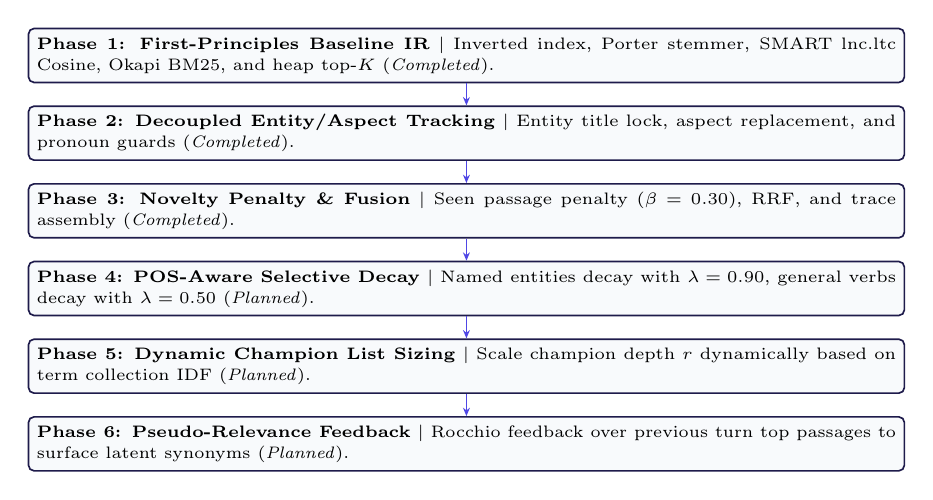
\begin{tikzpicture}[
    node distance=0.28cm,
    stage/.style={rectangle, draw=primarydark, fill=cardbg, rounded corners=2pt, font=\fontsize{6.5pt}{7.5pt}\selectfont\textsf, align=left, inner sep=3pt, text width=0.9\columnwidth, line width=0.6pt},
    arrow/.style={-{Stealth[length=3pt, width=2.5pt]}, line width=0.6pt, draw=accentblue}
]
    \node[stage] (p1) {\textbf{Phase 1: First-Principles Baseline IR} $\vert$ Inverted index, Porter stemmer, SMART $\text{lnc.ltc}$ Cosine, Okapi BM25, and heap top-$K$ (\textit{Completed}).};
    \node[stage, below=of p1] (p2) {\textbf{Phase 2: Decoupled Entity/Aspect Tracking} $\vert$ Entity title lock, aspect replacement, and pronoun guards (\textit{Completed}).};
    \node[stage, below=of p2] (p3) {\textbf{Phase 3: Novelty Penalty \& Fusion} $\vert$ Seen passage penalty ($\beta=0.30$), RRF, and trace assembly (\textit{Completed}).};
    \node[stage, below=of p3] (p4) {\textbf{Phase 4: POS-Aware Selective Decay} $\vert$ Named entities decay with $\lambda=0.90$, general verbs decay with $\lambda=0.50$ (\textit{Planned}).};
    \node[stage, below=of p4] (p5) {\textbf{Phase 5: Dynamic Champion List Sizing} $\vert$ Scale champion depth $r$ dynamically based on term collection IDF (\textit{Planned}).};
    \node[stage, below=of p5] (p6) {\textbf{Phase 6: Pseudo-Relevance Feedback} $\vert$ Rocchio feedback over previous turn top passages to surface latent synonyms (\textit{Planned}).};

    \draw[arrow] (p1) -- (p2);
    \draw[arrow] (p2) -- (p3);
    \draw[arrow] (p3) -- (p4);
    \draw[arrow] (p4) -- (p5);
    \draw[arrow] (p5) -- (p6);
\end{tikzpicture}
\caption{Six-phase development roadmap for TurnTrace.}
\label{fig:roadmap}
\end{figure}

% ==============================================================================
% 7. WORK DIVISION & AI-USE DECLARATION
% ==============================================================================
\section{Work Division \& AI-Use Declaration}
\label{sec:work_division}

\subsection{Team Ownership Matrix}
In accordance with hackathon instructions, Table~\ref{tab:work_division} outlines the functional component ownership across all four team members.

\begin{table}[H]
\centering
\scriptsize
\caption{Team Member Roles and Component Deliverables.}
\label{tab:work_division}
\begin{tabularx}{\columnwidth}{p{2.3cm} p{2.2cm} X}
\toprule
\textbf{Team Member} & \textbf{Component Track} & \textbf{Key Deliverables} \\
\midrule
\textbf{Shikhar Agarwal} \newline (2410110615) & \textbf{Indexing \& Data Preprocessing} & Corpus harvest (35k passages), tokenizer, Porter stemmer, multi-zone index, postings, champion lists. \\
\midrule
\textbf{Antra Agarwal} \newline (2410110404) & \textbf{Retrieval Engines \& Fusion} & SMART $\text{lnc.ltc}$ vector model, Okapi BM25, binary min-heap, Boolean engine, RRF fusion. \\
\midrule
\textbf{Bhupesh Bansal} \newline (2410110531) & \textbf{Conversational State Tracking} & Entity lock extractor, aspect state, decision detector, query rewriter, query decomposer. \\
\midrule
\textbf{Raghavendra Singh Sani} \newline (2410110465) & \textbf{Evaluation \& Trace Inspector} & Evaluation harness (13 systems), bootstrap/Wilcoxon tests, Express API, Trace Inspector UI. \\
\bottomrule
\end{tabularx}
\end{table}

\subsection{AI-Use Declaration}
In accordance with academic integrity guidelines:
\begin{enumerate}
    \item \textbf{AI Tools Utilized:} Google Antigravity IDE (Gemini coding agent) was used to assist in implementing boilerplate algorithms, unit test suites, and formatting scripts. Claude (Anthropic) was consulted for architectural validation and independent evaluation checks.
    \item \textbf{System Integrity:} \textbf{Zero external LLM or neural APIs are used during search runtime.} All indexing, scoring, decision detection, and trace assembly algorithms operate 100\% deterministically using pure Node.js code over inverted index collection statistics.
\end{enumerate}

% ==============================================================================
% REFERENCES
% ==============================================================================
\bibliographystyle{plain}
\bibliography{references}

% ==============================================================================
% APPENDIX (EXCLUDED FROM 8-PAGE LIMIT)
% ==============================================================================
\clearpage
\onecolumn
\appendix
\section*{Appendix}
\renewcommand{\thesubsection}{\Alph{subsection}}

\subsection{Detailed Mathematical Formulations}
\label{app:math}

\subsubsection{SMART Term Weighting Schemes}
Salton and Buckley's SMART notation specifies weight triples $\text{ddd.qqq}$ denoting document and query weighting conventions:
\begin{itemize}
    \item \textbf{Document Component (\texttt{lnc}):}
    \begin{align}
        \text{Term Frequency (\textbf{l}):} \quad tf_{\text{weight}} &= 1 + \ln(tf_{t,d}) \quad (\text{if } tf_{t,d} > 0, \text{ else } 0) \\
        \text{Document Frequency (\textbf{n}):} \quad idf_{\text{weight}} &= 1 \quad (\text{no collection frequency weighting applied to document}) \\
        \text{Cosine Normalization (\textbf{c}):} \quad w_{t,d} &= \frac{tf_{\text{weight}}}{\sqrt{\sum_{t' \in d} (tf_{\text{weight}, t'})^2}}
    \end{align}
    \item \textbf{Query Component (\texttt{ltc}):}
    \begin{align}
        \text{Term Frequency (\textbf{l}):} \quad tf_{\text{weight}} &= 1 + \ln(tf_{t,q}) \quad (\text{if } tf_{t,q} > 0, \text{ else } 0) \\
        \text{Document Frequency (\textbf{t}):} \quad idf_{\text{weight}} &= \ln(N / df_t) \\
        \text{Cosine Normalization (\textbf{c}):} \quad w_{t,q} &= \frac{tf_{\text{weight}} \cdot idf_{\text{weight}}}{\sqrt{\sum_{t' \in q} (tf_{\text{weight}, t'} \cdot idf_{\text{weight}, t'})^2}}
    \end{align}
\end{itemize}

\subsubsection{Reciprocal Rank Fusion Formulation}
Given candidate ranking lists $\{\mathcal{R}_1, \dots, \mathcal{R}_M\}$ produced by sub-queries:
\begin{equation}
    \text{RRF}(d) = \sum_{m=1}^M \frac{\mathbb{I}(d \in \mathcal{R}_m)}{60 + \text{rank}_m(d)}
\end{equation}
where $\text{rank}_m(d) \in \{1, \dots, K\}$ is the 1-based ordinal position of document $d$ in ranking $\mathcal{R}_m$.

\vspace{10pt}
\hrule
\vspace{10pt}

\subsection{Sample Execution Trace: Multi-Turn Conversation Inspection}
\label{app:trace}

Below is an authentic sample of the unredacted execution trace generated by TurnTrace during Conversation 3, Turn 2 (\textit{``Where is its orbit located in space?''}):

\begin{verbatim}
{
  "query": "Where is its orbit located in space?",
  "turnIndex": 2,
  "decision": {
    "action": "CARRY",
    "rationale": "Pronoun/anaphora guard triggered on pronoun 'its'; maintaining locked entity",
    "guards": {
      "pronounTriggered": true,
      "lockedEntityPreserved": true,
      "disjointCandidateDetected": false
    }
  },
  "context": {
    "lockedEntity": ["jame", "webb", "space", "telescop"],
    "entityLockMode": "hard_filter",
    "matchingCandidates": 100,
    "fallbackActive": false,
    "aspectTerms": [
      { "term": "orbit", "effectiveWeight": 1.000, "age": 0 },
      { "term": "locat", "effectiveWeight": 1.000, "age": 0 }
    ]
  },
  "rewrittenQuery": "Where is its orbit located in space? jame webb telescop",
  "provenance": [
    { "term": "orbit",    "role": "raw_query", "sourceTurn": 2, "weight": 1.0 },
    { "term": "locat",    "role": "raw_query", "sourceTurn": 2, "weight": 1.0 },
    { "term": "space",    "role": "raw_query", "sourceTurn": 2, "weight": 1.0 },
    { "term": "jame",     "role": "entity",    "sourceTurn": 1, "weight": 1.0 },
    { "term": "webb",     "role": "entity",    "sourceTurn": 1, "weight": 1.0 },
    { "term": "telescop", "role": "entity",    "sourceTurn": 1, "weight": 1.0 }
  ],
  "topResult": {
    "rank": 1,
    "docId": "doc_01716",
    "title": "James Webb Space Telescope - Section 3",
    "score": 0.4117,
    "termBreakdown": [
      { "term": "orbit",    "tf": 4, "queryWeight": 0.284, "docWeight": 0.312, "contrib": 0.0886 },
      { "term": "telescop", "tf": 3, "queryWeight": 0.211, "docWeight": 0.245, "contrib": 0.0517 },
      { "term": "webb",     "tf": 2, "queryWeight": 0.254, "docWeight": 0.198, "contrib": 0.0503 }
    ],
    "seenPenaltyApplied": false
  },
  "timings": {
    "normalizerMs": 0.42,
    "decisionMs": 0.31,
    "rewriterMs": 0.58,
    "retrievalMs": 3.84,
    "totalMs": 5.15
  }
}
\end{verbatim}

\vspace{10pt}
\hrule
\vspace{10pt}

\subsection{Core Algorithm Pseudocode}
\label{app:algorithms}

\subsubsection{Guarded Conversational Decision Detector}
\begin{verbatim}
Algorithm 1: Guarded Conversational Decision Detector
Input: Current query Q_k, Previous context state C_{k-1}, Candidate entities E_cand
Output: Action in {CARRY, ENTITY_SWITCH, RESET}, Updated entity E_k

1: PronounMatches <- ExtractPronouns(Q_k)
2: if PronounMatches is not empty then
3:    return (CARRY, C_{k-1}.lockedEntity)  // Guard 1: Anaphora override
4: end if

5: if AnyTokenIn(Q_k, C_{k-1}.lockedEntity) then
6:    return (CARRY, C_{k-1}.lockedEntity)  // Guard 2: Active entity token overlap
7: end if

8: TopTitles <- GetShallowTopTitles(Q_k, limit=3)
9: ValidNewEntity <- FindEntityInTitles(E_cand, TopTitles)

10: if ValidNewEntity is not null and ValidNewEntity != C_{k-1}.lockedEntity then
11:    if LexicalOverlap(Q_k, C_{k-1}.allTerms) > 0 then
12:       return (ENTITY_SWITCH, ValidNewEntity)
13:    else
14:       return (RESET, ValidNewEntity)
15:    end if
16: end if

17: return (CARRY, C_{k-1}.lockedEntity)
\end{verbatim}

\subsubsection{Seen-Passage Penalty Scoring}
\begin{verbatim}
Algorithm 2: Seen-Passage Penalty Scoring
Input: Candidate ranked documents D = [d_1, ..., d_M], Session seen history S_seen, Penalty beta = 0.30
Output: Re-ranked top-K documents R_K

1: for each d in D do
2:    if d.docId in S_seen then
3:       d.score <- d.score * (1.0 - beta)  // Demote previously exposed passages
4:       d.seenPenaltyApplied <- true
5:    else
6:       d.seenPenaltyApplied <- false
7:    end if
8: end for

9: Sort D in descending order of d.score
10: R_K <- D[1 .. K]
11: for each d in R_K do
12:    S_seen.add(d.docId)  // Record top-K displayed passages for future turns
13: end for
14: return R_K
\end{verbatim}

\end{document}
